\section[LPUS system]{LPUS system}

In this section, we elaborate on the two LPUS components that the LPUS system
consists of, the kernel driver and the user application. We go through the
steps LPUS makes to enable live forensics and how LPUS can perform live
forensics without extracting the memory file. For convention, the kernel driver
will be called the \textbf{backend} and the user application will be called the
\textbf{frontend}. Here are the steps that LPUS takes from startup to
termination. (1) LPUS registers the registry keys and \textbf{loads the kernel
driver in the system}. (2) LPUS downloads and \textbf{loads the debug symbols}
on the current system.  (3) LPUS \textbf{finds the kernel base address}. (4)
LPUS uses the kernel base address to \textbf{perform forensics}. (5) LPUS
terminates. We will go through each step and analyze what LPUS does.

\subsection[Loading driver]{Loading driver}

LPUS loads the kernel driver on startup. Loading the kernel driver requires a
registry key containing the path to the driver and the load driver privilege
enabled. LPUS writes the registry key at
\texttt{HKEY\_LOCAL\_MACHINE\textbackslash System \textbackslash
CurrentControlSet \textbackslash Services \textbackslash lpus} with the
\texttt{ImagePath} value contains the path to the kernel driver as shown in
Figure \ref{fig:registry}. This registry key will be passed onto
\texttt{NtLoadDriver} as the first parameter to load the driver. To make the
driver loading success, LPUS will enable the \texttt{SeLoadDriver} privilege.
The \texttt{SeLoadDriver} is available if the user running LPUS is an
Administrator, however, the value is disabled. LPUS uses the code on Listing
\ref{lst:seloaddriver} to enable the privilege. After these operations, LPUS
has loaded the kernel driver onto the running system


\begin{figure}[h]
  \centering
  \caption{LPUS setup registry}
  \label{fig:registry}
  \includegraphics[scale=1]{images/registry.png}
\end{figure}

\begin{lstlisting}[language=rust,caption={Enable SeLoadDriver},label={lst:seloaddriver},float,floatplacement=H]
let str_se_load_driver_privilege = CString::new("SeLoadDriverPrivilege")
                                   .unwrap();
let mut token_handle: HANDLE = null_mut();
let mut luid = LUID::default();
OpenProcessToken(
    GetCurrentProcess(),
    TOKEN_ADJUST_PRIVILEGES,
    &mut token_handle,
);
LookupPrivilegeValueA(null_mut(),
                      str_se_load_driver_privilege.as_ptr(),
                      &mut luid);
let mut new_token_state = TOKEN_PRIVILEGES {
    PrivilegeCount: 1,
    Privileges: [LUID_AND_ATTRIBUTES {
        Luid: luid,
        Attributes: SE_PRIVILEGE_ENABLED,
    }],
};
AdjustTokenPrivileges(
    token_handle,
    0,
    &mut new_token_state,
    16,
    null_mut(),
    null_mut(),
);
CloseHandle(token_handle);
\end{lstlisting}

\subsection[Load debug symbols]{Load debug symbols}

After successfully loading the kernel driver, LPUS will download the debug
symbols for the system. LPUS parse the GUID and age for the kernel file
\texttt{C:\textbackslash \textbackslash Windows \textbackslash System32
\textbackslash ntoskrnl.exe} and builds the URL to download the PDB from the
Microsoft server as in Listing \ref{lst:downloadpdb}. After the file is
downloaded, LPUS uses a third-party PDB module to parse the downloaded PDB file
into a hashmap to index quickly. There are two hashmaps, the hashmap of global
variables and functions, and the hashmap of structure and members. The hashmap
of global variables and functions are indexed by the name of the symbol and
stores the offset to the symbol. For the hashmap of structures, the index key
is the structure name and stores the hashmap of members. The hashmap of a
member is indexed by the member name and stores the member's type and offset of
the member in the structure. Listing \ref{lst:pdbstore} shows the data
structure the debug symbols are stored.

\begin{lstlisting}[language=rust,caption={Stores debug symbols},label={lst:pdbstore},float,floatplacement=H]
// Symbol name -> Offset
type SymbolStore = HashMap<String, u64>;

// Struct name -> Hashmap(Member -> (Type, Offset))
type StructStore = HashMap<String, HashMap<String, (String, u64)>>;

struct PdbStore {
    pub symbols: SymbolStore,
    pub structs: StructStore,
}
\end{lstlisting}

\subsection[Setup communication and kernel base address]{Setup communication and kernel base address}

After loading the kernel driver and debug symbols, LPUS setups the connection
between the backend and frontend and search for the kernel base address. The
connection between the two is vital, and this is what makes LPUS capable of
querying the kernel space.

The backend and frontend communication is kernel-land and user-land
communication. The kernel-land cannot access the user-land and the user-land
cannot access the kernel land. To communicate with each other, they must have a
shared object, a physical file. Communicating using this physical file is the
same as socket programming between the server and a client. The packet is sent
by the user application in the form of an IRP. The driver receives the IRP and
the driver performs computation depends on the IRP action code.  Sending data
between the two also uses the IRP packet. The protocol must first be defined by
the user application to send or receive. There are four modes for transferring
data: \textit{in direct} for sending data to the driver, \textit{out direct}
for receiving data from the driver, neither for communication without data
transferring and bi-directional if the user application sends to and receives
from the driver.

To create the communication, the driver creates the physical file and user
application \textit{binds}, connect, to the file. Both frontend and backend
have to accept the set of action codes and data input-output to avoid crashing
the system. After that, the user application can call \texttt{DeviceIoControl}
to send the action code, the input buffer, the output buffer to the driver. The
code setting up the communication can be found on Listing \ref{lst:deviceio}.

\begin{lstlisting}[language=cpp,caption={Setup communication},label={lst:deviceio},float,floatplacement=H]
// Driver code
NTSTATUS
DriverControl(PDEVICE_OBJECT /* DriverObject */, PIRP Irp) {
  PIO_STACK_LOCATION irpSp = IoGetCurrentIrpStackLocation(Irp);
  ULONG controlCode = irpSp->Parameters.DeviceIoControl.IoControlCode;
  switch (controlCode) {
    // handle action
  }
}

NTSTATUS
DriverEntry(
    _In_ PDRIVER_OBJECT     DriverObject,
    _In_ PUNICODE_STRING    /* RegistryPath */
) {
  // ntUnicodeString   = "\\Device\\lpus"
  // ntWin32NameString = "\\DosDevices\\lpus"

  // creates the file device
  IoCreateDevice(
    DriverObject,             // Our Driver Object
    0,                        // We don't use a device extension
    &ntUnicodeString,         // Device name "\Device\lpus"
    FILE_DEVICE_UNKNOWN,      // Device type
    FILE_DEVICE_SECURE_OPEN,  // Device characteristics
    FALSE,                    // Not an exclusive device
    &deviceObject);           // Returned ptr to Device Object

  // make the file accessible from user space
  IoCreateSymbolicLink(&ntWin32NameString, &ntUnicodeString);

  // register function receiving IRP
  DriverObject->MajorFunction[IRP_MJ_DEVICE_CONTROL] = DriverControl;
}

// User application code
HANDLE f = CreateFile("\\\\.\\poolscanner", ...);
DeviceIoControl(f, controlCode, ...);
\end{lstlisting}

When the connection between the backend and frontend is established, the
frontend will send some required offset for the backend to get the kernel base
address.  To get the kernel base address, LPUS uses the process list. The
offset from the kernel base address to the process list head can be fetched
from debug symbols, with the address of the process list we can easily
calculate the kernel base address. This requires us to find the process list
head. The backend can get inside the process list by getting an
\texttt{\_EPROCESS} through calling \texttt{IoGetCurrentProcess}. From a node
inside the list, LPUS can search for the head by traversing through the list.
Unfortunately, this does not work so well, and the process list is a circular
linked list, there is no null at the end or at the front of the list, which
makes it challenging to find the head.  However, we have noticed an interesting
fact with \texttt{IoGetCurrentProcess}.  The process returned by calling
\texttt{IoGetCurrentProcess} is the process of interacting with the driver, and
the process loading the driver onto the system is the \texttt{System} process.
The \texttt{System} process, how convenient, is the first item in the process
list. By getting the \texttt{System} when the driver loads using
\texttt{IoGetCurrentProcess}, we only need to traverse back one time to get the
list head. When the list head address is found, a subtraction from the offset
parsed from the PDB file will result in the kernel base address. The backend
will now return the kernel base address to the frontend.

\subsection[Perform forensics]{Perform forensics}

Reaching this step, LPUS has successfully loaded the kernel driver in the
system space, prepared the debug symbols, set up the communication between the
backend and userland, and have the kernel base address. From now, LPUS can
perform forensics on the system.

With the kernel base address, LPUS can easily get and traverse every list,
inspect any global variable if the type of the variable is well-known. The list
of processes LPUS can access is \texttt{PsActiveProcessHead},
\texttt{KiProcessListHead}, and the \texttt{HandleTableListHead}. LPUS can
access the kernel list by reading \texttt{PsLoadedModuleList}. The SSDT table
can be accessed by reading \texttt{KiServiceTable}, as well as the unloaded
module list in \texttt{MmUnloadedDrivers}.

Pool tag scanning is feasible with LPUS. As shown in Table \ref{tab:nonpaged},
the start and end section of the non-paged pool are indexed by the kernel base
address. LPUS can easily fetch the range value and perform scanning in between
looking for four-byte value. Scanning in this region is safe, but we should
take precautions. The address in this region is virtual memory, some pages are
mapped in RAM, but some pages do not. Accessing the address where the page is
not in RAM will cause the system to crash with a violation \texttt{Page Fault
In Nonpaged Area}. LPUS tries to handle the situation by checking every page
aligned address before accessing the page. The page aligned address will be
checked using \texttt{MmIsAddressValid}. If the result is false, or the address
is invalid, this indicates the page starting at the address is not assigned a
physical page. LPUS skips a page on \texttt{MmIsAddressValid} returns false,
and other cases where the memory accessed passes the current page but the next
page is invalid.

Because LPUS possesses the kernel base address, LPUS can explore the kernel
space if it knows the exact address of kernel variables and follows the
pointers inside kernel structures. With this forensics possibility, we show
more on what LPUS can do in Chapter 7.

\subsection[Termination]{Termination}

After forensics is done, LPUS closes the physical file, unloads the driver, and
terminates itself. A trace to the LPUS kernel driver remains in the unloaded
driver list.

The LPUS system's abstract view on Performing Forensic step is described in
Figure \ref{fig:lpus}. The controller in the frontend emits a request to the
kernel (1) for variable value or pool tag scanning. The driver in the back end
will resolve the result (2) in kernel space and return (3) to the front end.
Then the Result Handler will handle (4) the returned result, whether to
continue querying the system or print to the console. The PdbStore is used to
give the exact offset to variables and structure members.  All communication
between the backend and frontend is done through DeviceIoControl hence the two
device ``\textbackslash Device\textbackslash lpus'' and ``\textbackslash
DosDevice\textbackslash lpus''

\begin{figure}[h]
  \centering
  \caption{LPUS Performing Forensics}
  \label{fig:lpus}
  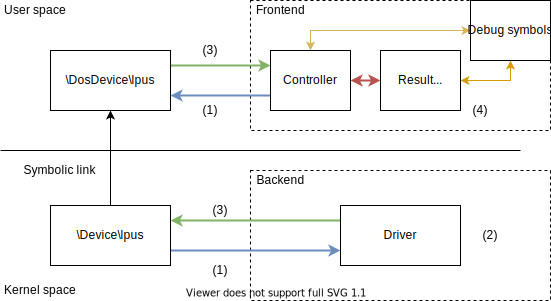
\includegraphics[scale=0.7]{images/lpus.png}
\end{figure}
